\section{Demonstration des Programms}

\begin{frame}{Umsetzung}
	%\begin{minipage}[t]{0.35\textwidth}
	%	\centering
	%	
\includegraphics[width=\textwidth]{images/qt-logo.png}
	%\end{minipage}
	%\hfill
	%\begin{minipage}[t]{0.35\textwidth}
	%	\centering
	%	
\includegraphics[width=\textwidth]{images/c++-logo.png}
	%	\vskip 1em
	%	
\includegraphics[width=\textwidth]{images/qcp-logo.png}
	%\end{minipage}
	
	\begin{columns}[T] % align columns{\tiny }
		\begin{column}{0.3\textwidth}
			\centering
			
\includegraphics[width=\textwidth]{images/c++-logo.png}
		\end{column}
		\hfill
		\begin{column}{0.3\textwidth}
			\centering
			
\includegraphics[width=\textwidth]{images/qt-logo.png}
		\end{column}
	\end{columns}
	\vskip 1.5em
	\begin{figure}
		\centering
		
\includegraphics[scale=0.5]{images/qcp-logo.png}
	\end{figure}

\end{frame}



\begin{frame}{\insertsection}
\end{frame}

\begin{frame}{\insertsection}
	\begin{figure}
		%\animategraphics[autoplay,loop,width=\linewidth]{30}{images/GIFs/cantina/cantina-}{1}{827}
		\caption*{Applikation \it{Wavedit}, Github: \href{https://github.com/gooosz/Wavedit.git}{https://github.com/gooosz/Wavedit.git}}
	\end{figure}
\end{frame}

% Nochmal als Bilder falls Gif zu schnell für Erklärungen war
\begin{frame}{\insertsection}
	\begin{figure}
		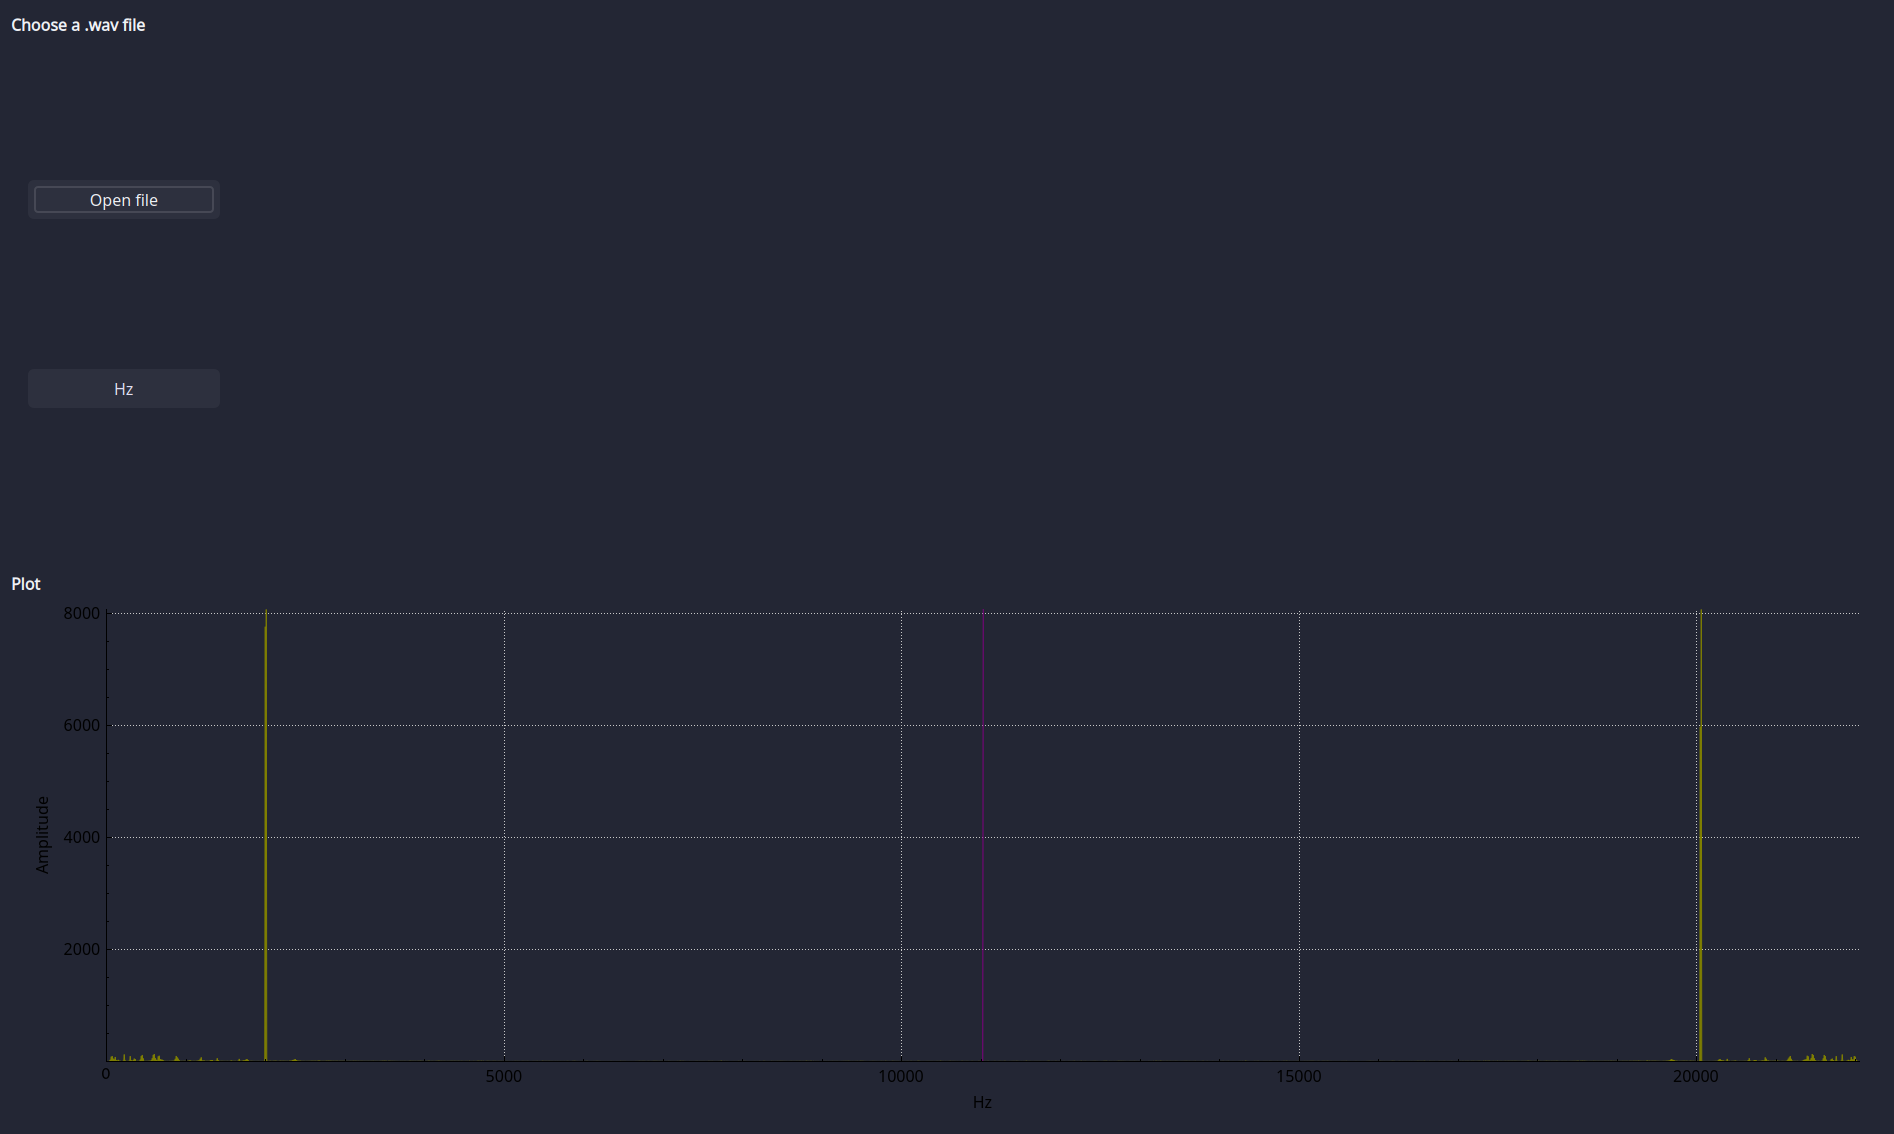
\includegraphics[width=\linewidth]{images/sin+cantina.png}
		\caption*{Frequenzspektrum von WAV Datei}
	\end{figure}
	% click on Play button to play the shown wav file
	\sound[]{Play audio}{audio/Sin440Hz_CantinaBand3.wav}
	%\sound[]{Play audio}{audio/sin750Hz-StarWars3.wav}
\end{frame}
\begin{frame}{\insertsection}
	\begin{figure}
		\includegraphics[width=\linewidth]{images/sin+cantina\_filtered.png}
		\caption*{Frequenzspektrum nach Filtern von $\SI{2000}{\hertz}$ in WAV Datei}
	\end{figure}
	% click on Play button to play the shown wav file
	\sound[]{Play audio}{audio/Sin440Hz_CantinaBand3.wav_filtered2007.87Hz.wav}
	%\sound[]{Play audio}{audio/sin750Hz-StarWars3.wav_filtered759.08Hz.wav}
\end{frame}
